\documentclass[10pt,a4paper]{report}
\usepackage[utf8]{inputenc}
\usepackage[T1]{fontenc}
\usepackage{tabularx}
\usepackage{graphicx}
\usepackage{enumitem}
\usepackage{lmodern}
\usepackage{textcomp}
\usepackage{booktabs}
\usepackage{longtable}
\usepackage{titlesec}
\setcounter{secnumdepth}{4}
\usepackage{rotating}
\usepackage{array}
\usepackage{makecell}
\usepackage{multirow}
\usepackage[dvipsnames,table,xcdraw]{xcolor}
\usepackage{hhline}
\usepackage{caption}
\usepackage{verbatim}
\usepackage{longtable}
\graphicspath{{./Immagini/}}
\renewcommand*\contentsname{\textbf{Index}}
\usepackage{hyperref}
\hypersetup{colorlinks=true,linkcolor=black}
\usepackage{titletoc}
\usepackage{etoolbox}
\usepackage{lettrine}
\usepackage{geometry}
\usepackage{listings}
\geometry{
 a4paper,
 total={170mm,257mm},
 left=20mm,
 top=15mm,
 }
\makeatletter
\patchcmd{\chapter}{\if@openright\cleardoublepage\else\clearpage\fi}{}{}{}
\makeatother
\titleformat*{\section}{\centering\normalfont\Large\bfseries}
\usepackage{color}

\definecolor{mygreen}{rgb}{0,0.6,0}
\definecolor{mygray}{rgb}{0.5,0.5,0.5}
\definecolor{mymauve}{rgb}{0.58,0,0.82}

\lstset{ 
  backgroundcolor=\color{white},   % choose the background color; you must add \usepackage{color} or \usepackage{xcolor}; should come as last argument
  basicstyle=\footnotesize,        % the size of the fonts that are used for the code
  breakatwhitespace=false,         % sets if automatic breaks should only happen at whitespace
  breaklines=true,                 % sets automatic line breaking
  captionpos=b,                    % sets the caption-position to bottom
  commentstyle=\color{mygreen},    % comment style
  deletekeywords={...},            % if you want to delete keywords from the given language
  escapeinside={\%*}{*)},          % if you want to add LaTeX within your code
  extendedchars=true,              % lets you use non-ASCII characters; for 8-bits encodings only, does not work with UTF-8
  frame=single,                       % adds a frame around the code
  keepspaces=true,                 % keeps spaces in text, useful for keeping indentation of code (possibly needs columns=flexible)
  keywordstyle=\color{blue},       % keyword style
  language=Octave,                 % the language of the code
  morekeywords={*,...},            % if you want to add more keywords to the set
  numbers=left,                    % where to put the line-numbers; possible values are (none, left, right)
  numbersep=5pt,                   % how far the line-numbers are from the code
  numberstyle=\tiny\color{mygray}, % the style that is used for the line-numbers
  rulecolor=\color{black},         % if not set, the frame-color may be changed on line-breaks within not-black text (e.g. comments (green here))
  showspaces=false,                % show spaces everywhere adding particular underscores; it overrides 'showstringspaces'
  showstringspaces=false,          % underline spaces within strings only
  showtabs=false,                  % show tabs within strings adding particular underscores
  stepnumber=1,                    % the step between two line-numbers. If it's 1, each line will be numbered
  stringstyle=\color{mymauve},     % string literal style
  tabsize=2,                       % sets default tabsize to 2 spaces
  title=\lstname                   % show the filename of files included with \lstinputlisting; also try caption instead of title
}
\usepackage{sectsty}
\sectionfont{\bfseries\Large\raggedright}
\usepackage[Lenny]{fncychap}

\begin{document}
\linespread{1,28}
\sffamily
\begin{titlepage}
\begin{center}
\normalsize

\begin{center}

\begin{tabular}[t]{@{} l @{} c @{} r @{}}
\parbox[c]{0.15\textwidth}{\raggedright 
\includegraphics[width=0.15\textwidth]{logo}}
&
\parbox[c]{0.7\textwidth}
{
\centering \bfseries
University of L'Aquila \\[-5pt]
\rule{0.6\textwidth}{1pt} \\
{\centering \scshape \small Department of Engineering and \\Information Science and Mathematics} \\}
&
\parbox[c]{0.15\textwidth}{\raggedleft 
\includegraphics[width=0.15\textwidth]{disim}}
\end{tabular}
\end{center}

\bigskip \bigskip



\bigskip
\bigskip
\bigskip

\vfil

{\bfseries \large
Report Homework \#1 \\}
{\bfseries \Large
Water Distribution, Leakage and Quality Control System
}

{\large
\bigskip
\bigskip
\bigskip
\bigskip
{\bfseries \large Professor \\ }
\bigskip
\textbf{Prof.} \textit{Vittorio Cortellessa} \\
}

{\large
\bigskip
\bigskip
\bigskip
\bigskip
{\bfseries \large Students \\ }
\bigskip
\textit{Gaetano Fichera \& Giovanni Lezzi} \\
}

\vfil
\vfil

\vspace{2\baselineskip}

{\large
\bigskip
\bigskip
\bigskip
\bigskip
{\bfseries \large Github Project Repository: \\ }
\bigskip
\textit{\href{https://github.com/GaetanoFichera/Water-Quality-Control-System}{https://github.com/GaetanoFichera/Water-Quality-Control-System}} \\
}

\vfil \vfil \vfil

\rule{\textwidth}{1pt}\\
{\scshape Academic Year 2017-2018}

\end{center}
\end{titlepage}
\tableofcontents{}
\newpage
\chapter{\textbf{Our Homework}}

The task in this second homework is to create a Performance Model based on the system that we have modeled in the first homework. Using the Sequence Diagrams, we built the Execution Graph, and, through the Deployment Diagram we have built a Queueing Network. From the analysis of the Execution Graph we obtained the Demand Vectors that we used to parameterize the Queueing network. After that, the network has been
resolved through a tool in order to obtain the output parameters that would allow to evaluate the system performance.
In the final phase through the Architectural Description Language Aemilia we had the possibility to have a further evaluation of the system's performance.
\chapter{\textbf{Work Planning}}

The workflow was:

\begin{itemize}
	\item Light rework on our UML Model;
	\item Study of theoretical concepts of Queuing Networks and how to 			create the Execution Graph from Sequence Diagram;
	\item Connection between Deployment and Component Diagram;
	\item Drafting of the Executiong Graph;
	\item Calculation of the consumption of physical resources in an 			overhead matrix;
	\item Drafting of the Queueing Network;
	\item Performance Analysis and evaluation, and Refactoring of the 			Queueing Network Model;
	\item Study of Aemilia;
	\item Drafting of the State Diagrams for the implementation in 				Aemilia;
	\item Drafting of the Flow Graph;
	\item Performance analysis in Aemilia;	
\end{itemize}


\chapter{\textbf{Light Rework On Our UML Model}}

After serious consideration of our last homework, we noticed that there were failures. Below is a list of rework:

\begin{itemize}
	\item We have applied the stereotypes to the Communication Paths 		within the Deployment Diagram;
	\item in order to improve system performance and to better 				stratify the deployment, we decided to add 3 new nodes: 
	\begin{itemize}
	\item "SeaweedPickingInlandControlUnit";
	\item "Seaweed Picking Outgoing Control Unit";
	\item "MagikarpControlUnit".
	\end{itemize}					 
	and , for this purpose we have also inserted a new profile called 		"Control Unit" from the	server 	stereotype, these 3 new nodes are 		connected to the server with a wired connection and to sensors 			with a wireless connection;
	\item For the connections between the Control Center Server and 		the	two Inland and Outgoing Seaweed Picking Control Units we 			have inserted a new communication path stereotype that does 			not consume resources because when we started the modeling 				work for the Queueing Network we considered the two Control 			Units located in the same physical space as the Control 				Center Server, then we use a "Internal Connection" stereotype with 	zero consumption of resources;
	\item We have added the operations to the components subsequently 		reused in the Sequence Diagram, not done in the first homework;
	\item we realized the lack of an internal server to the Control 		Center 	Pomezia that managed the requests coming from the App 			inside it;
	\item we realized that in the sequence diagram "check quality" the 	call from the component "check quality parameters inland /				outgoing" was missing to the component "parameters Quality 				archieve" to retrieve the desired water parameters;
	\item we have established the types of connections between one 			node and the other of the deployment diagram, obtaining:
	
	\begin{itemize}
		\item between the Control Center Server and the two Apps a 				Wired Connection;
		\item between Control Center Server and Seaweed Picking a 				Wireless Connection;
		\item between the Control Center Server and the Water Company 			Server and the Purification System Center an Internet 					Connection.
	\end{itemize}

	\item we have agreed that there is a single database that is 			connected to the water company server;
	\item we realized that in the water sampling phase, the sensors 		will send the data of the water samples to the Control Center 			Server which, in turn, using the sample archieve component will 		send the data to the water company server, the problem is that in 		the SD 	after the component sample archive is not invoked any 			component that refers to the water company server. Solution:
	\begin{itemize}
	\item We have decided to add a component called "Sample Archive" 		to the water company server which is responsible for saving data 		on the DB. In going to add this correction we realized 	that in			fact we have failed to use sample sender. Then we have made a 			small change: 
	\begin{itemize}
		\item sample sender is inside 	the control center server;
		\item sample archive is located inside the water company 				server and	manages the data on the db.
		\end{itemize}
	\end{itemize}	
	\item We modified the sequence diagram of "StartUpSamplingWater" 		as 	we realized that the component sample data on the 					SeadweedPIckingInland / Outgoing node communicated with the 			"SampleSender" component on the ControlCenterServer node.
\end{itemize}

Below you can find the description of the new profiles popping out.

\section{Wired Connection Profile}

\begin{longtable}{|p{4cm}|p{9cm}|}

\hline
\textbf{Wired Connection} & \\


\hline
Metamodel Class & Communication Path\\

\hline
Description & It is a representation of the physical meaning of Wired Connection\\

\hline
Tagged Values & \\

\hline
Constraints &\\

\hline
\end{longtable}
  
\section{Internet Connection Profile}

\begin{longtable}{|p{4cm}|p{9cm}|}

\hline
\textbf{Internet Connection} & \\


\hline
Metamodel Class & Communication Path\\

\hline
Description & It is a representation of the physical meaning of Internet Connection\\

\hline
Tagged Values & \\

\hline
Constraints &\\

\hline
\end{longtable}

\section{Wireless Connection Profile}

\begin{longtable}{|p{4cm}|p{9cm}|}

\hline
\textbf{Wireless Connection} & \\


\hline
Metamodel Class & Communication Path\\

\hline
Description & It is a representation of the physical meaning of Wireless Connection\\

\hline
Tagged Values & \\

\hline
Constraints &\\

\hline
\end{longtable}

\section{Internal Connection Profile}

\begin{longtable}{|p{4cm}|p{9cm}|}

\hline
\textbf{Internal Connection} & \\


\hline
Metamodel Class & Communication Path\\

\hline
Description & It is a representation of the physical meaning of Internal Connection\\

\hline
Tagged Values & \\

\hline
Constraints &\\

\hline
\end{longtable}

\section{Control Unit Profile}

\begin{longtable}{|p{4cm}|p{9cm}|}

\hline
\textbf{Internal Connection} & \\


\hline
Metamodel Class & Node\\

\hline
Description & It is a representation of the physical meaning of Control Unit\\

\hline
Tagged Values & \\

\hline
Constraints &\\

\hline
\end{longtable}
\chapter{\textbf{Use Cases Decision}}

In building the Performance Model we considered only two use cases. To satisfy the Homework request the Use cases choosen are:
\begin{itemize}
	\item StartUp Sampling Water activated by Sample Supervisor;
	\item Check Water Quality activated by Quality Control Supervisor.
\end{itemize}

\chapter{\textbf{Identification Of Performance Requirements}}


The following consideration has been made: \\
one kilometer of the route with respect to the connection point with the system is taken into account for an Entry Water Channel or Exit of 5 meters radius, and every 10 meters must be 10 Seaweed Picking, with a total of 1000 Seaweed Picking. \\
Non-functional requirements are:
\begin{itemize} 
	\item Each sensor must take 10 ms to carry out a sampling;
		\item The time between a sampling and an other is 60 s;
	\item The Utilization of each node must be less than 90\%;
	\item The response time of an Actor Task must not exceed 300 ms specifically referenced to "CheckWaterQuality" Use Case.
\end{itemize} 

\newpage \chapter{\textbf{Development Of Component Diagram Into Deployment Diagram}}

\newpage \chapter{\textbf{Model WCS With Execution Graphs}}

The Use Cases we have considered are:
\begin{itemize}
\item UC1 StartUp Sampling Water activated by Sample Supervisor;
\item UC3 Check Water Quality activated by Quality Control Supervisor.
\end{itemize}
In reference to the Use Cases taken into consideration, to better understand our architecture, we have combined the Deployment Diagram with Component Diagram. In the figure below this is represented.

\begin{center}
  \makebox[\textwidth]{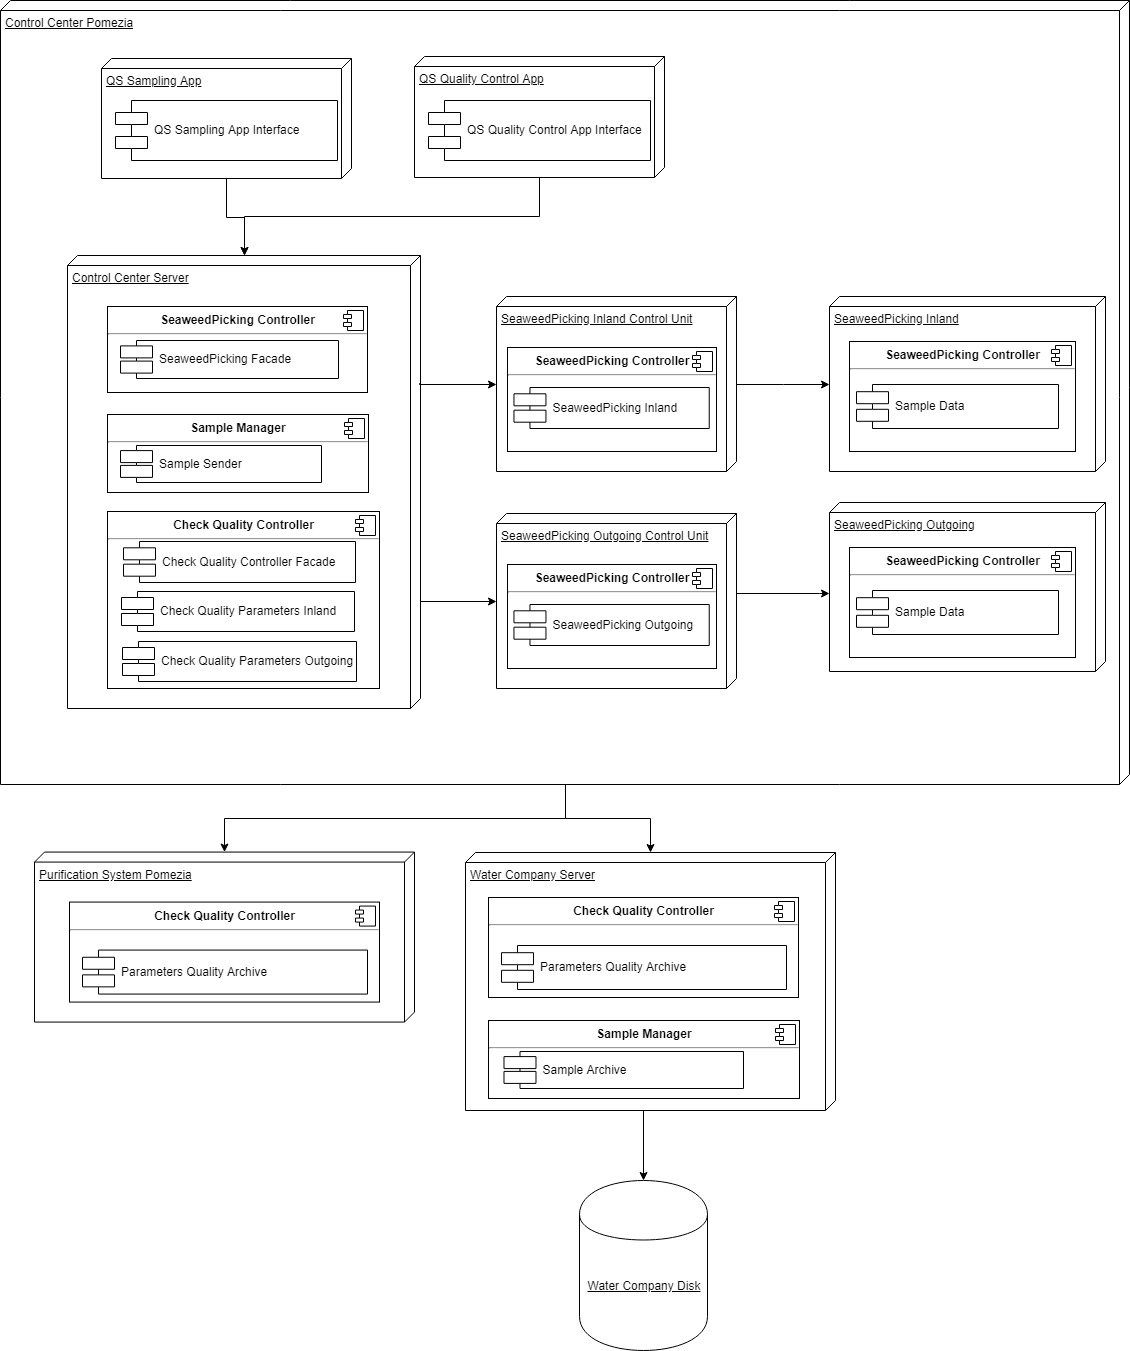
\includegraphics[width=\textwidth]{DeploymentDiagramEComponentDiagram.jpg}}
\end{center}
\bigskip
\captionof{figure}{Deployment Diagram + Component Diagram}

\newpage \section{Demand Vector}

Il Demand Vector scelto in base alle risorse virtuali che risaltano dal deployment diagram sono: 

\begin{longtable}{|p{4cm}|p{9cm}|}

\hline
\textbf{
Wired Connection Request} & \\

\hline
\textbf{Wireless Connection Request} & \\

\hline
\textbf{Internet Connection Request} & \\

\hline
\textbf{Database Request} & \\

\hline
\textbf{Control Center Server CPU} & \\

\hline
\textbf{Water Company Server CPU} & \\

\hline
\textbf{Purification System Pomezia CPU} & \\

\hline
\textbf{Seaweed Picking Inland Control Unit CPU} & \\

\hline
\textbf{Seaweed Picking Outgoing Control Unit CPU} & \\

\hline
\textbf{Seaweed Picking Outgoings Sample Request} & \\

\hline
\textbf{Seaweed Picking Inlands Sample Request} & \\

\hline
\end{longtable}

\textbf{Spiegare cosa sono queste risorse virtuali}\\
\newpage

The Execution Graphs obtained are:

\begin{itemize}
\item UC1 Sampling Water activated by Sample Supervisor:
	\bigskip
	\bigskip
	\begin{center}
 	 \makebox[\textwidth]{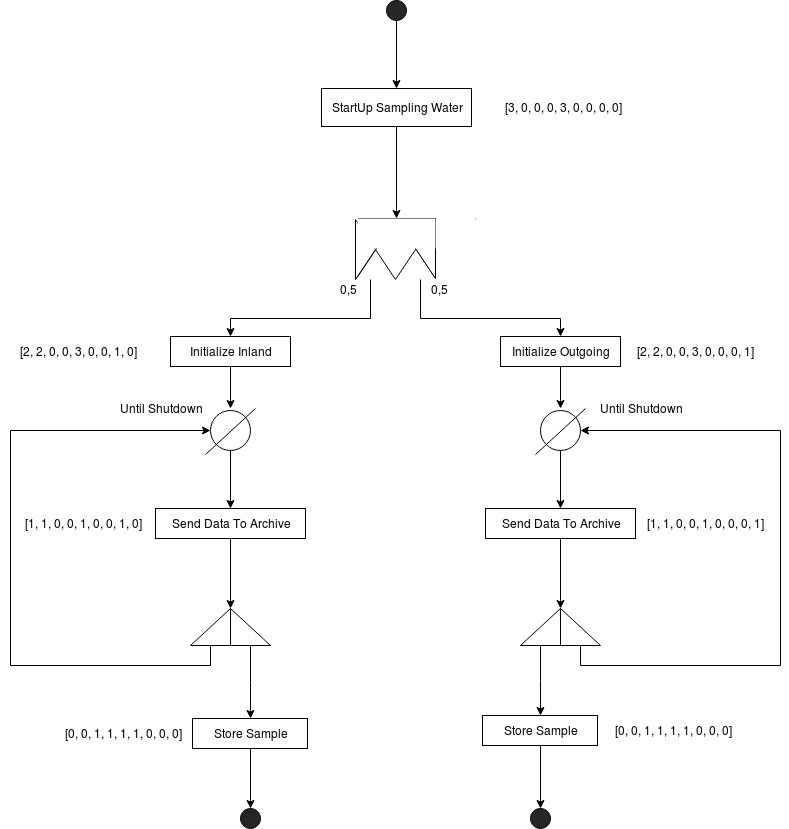
\includegraphics[width=\textwidth]				{EGUC1StartUpSamplingWater.jpg}}
	\end{center}
	\bigskip
	\captionof{figure}{EG UC1 StartUp Sampling Water}
\newpage
\item UC3 Check Water Quality activated by Quality Control Supervisor:
	\bigskip
	\bigskip
	\bigskip
	\bigskip
	\begin{center}
 	 \makebox[\textwidth]{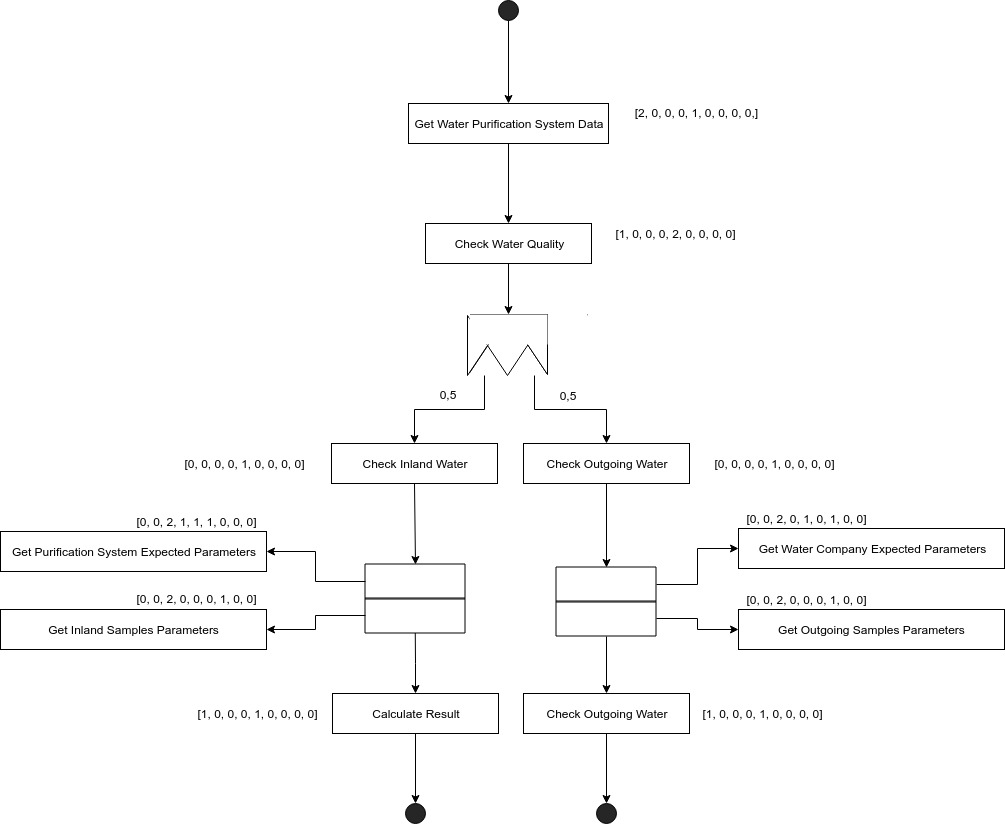
\includegraphics[width=\textwidth]				{EGUC3CheckWaterQuality.jpg}}
	\end{center}
	\bigskip
	\captionof{figure}{EG UC3 Check Water Quality}
\end{itemize}




\newpage \chapter{\textbf{Queueing Network Model}}

Then we have identified the physical nodes of our system going to introduce how the Execution Graphs are connected to them:
\bigskip
\bigskip
\bigskip
\bigskip
\begin{center}
\makebox[\textwidth]{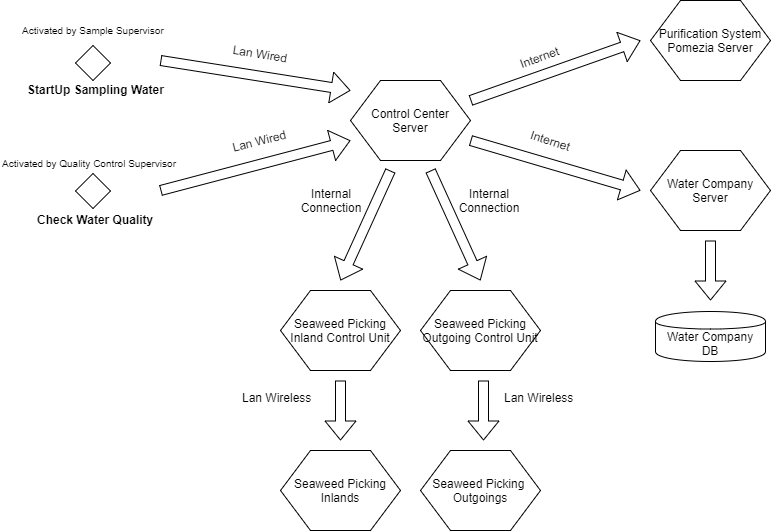
\includegraphics[width=\textwidth]				{PhysicalNodes.png}}
\end{center}
\bigskip
\captionof{figure}{Physical Nodes}

\newpage
This is the Queueing Network so obtained:
\bigskip
\begin{center}
\makebox[\textwidth]{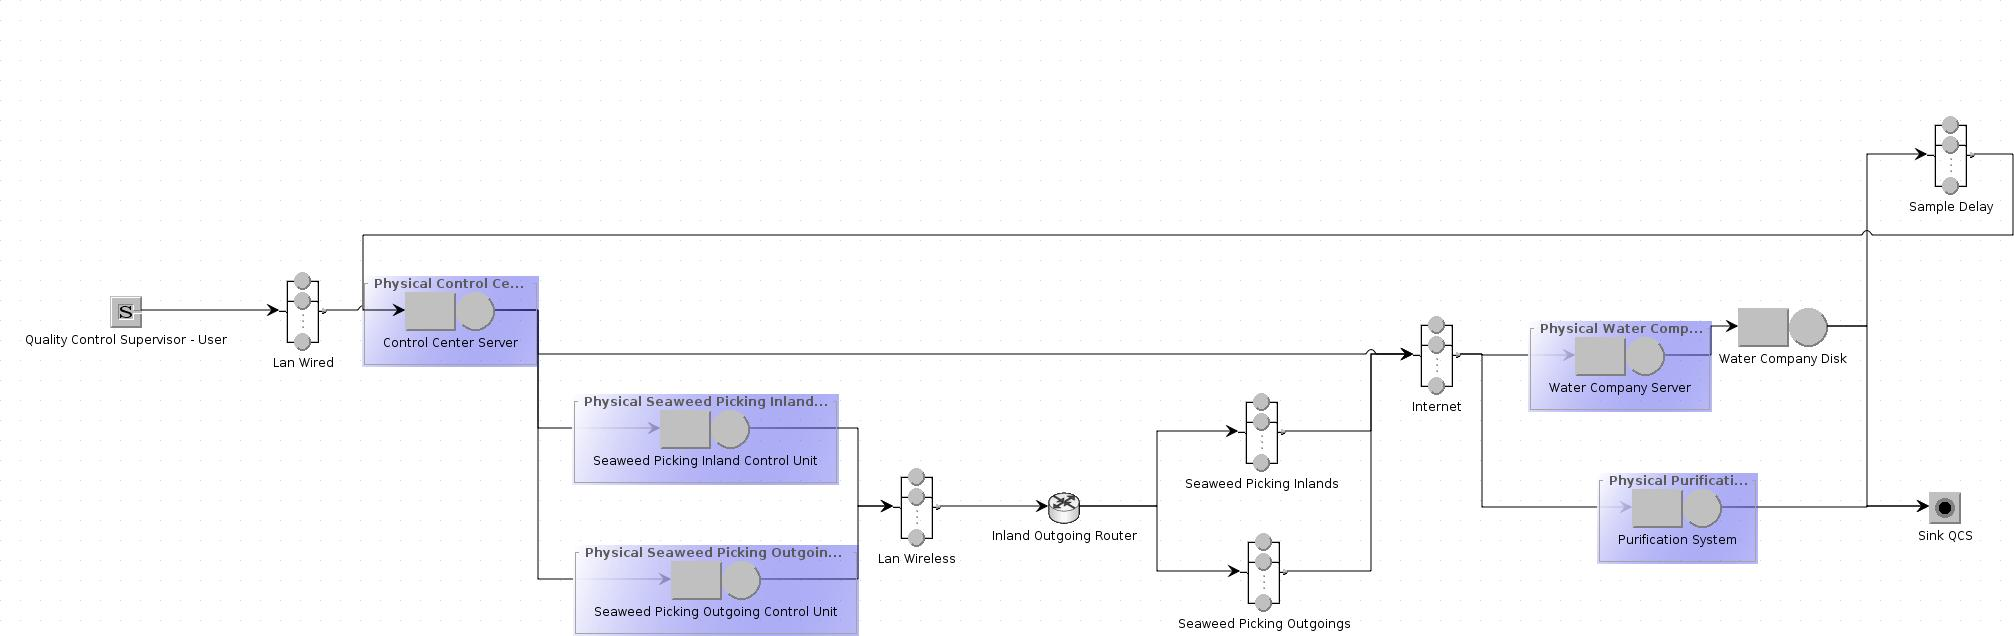
\includegraphics[width=\textwidth]				{QueueingNetwork.jpg}}
\end{center}
\bigskip
\captionof{figure}{Queueing Network}

\bigskip
After several tests, we agreed to reduce the sampling time to 500 seconds to refine the performance analysis. On jmt for the same reason we have only one SeaweedPicking Control Unit and no two for In / Out.\\
We have also decided to eliminate the finite capacity regions as useless for the purposes of our project. So our final Queueing Network has become this:
 
\bigskip
\bigskip
\bigskip
\begin{center}
\makebox[\textwidth]{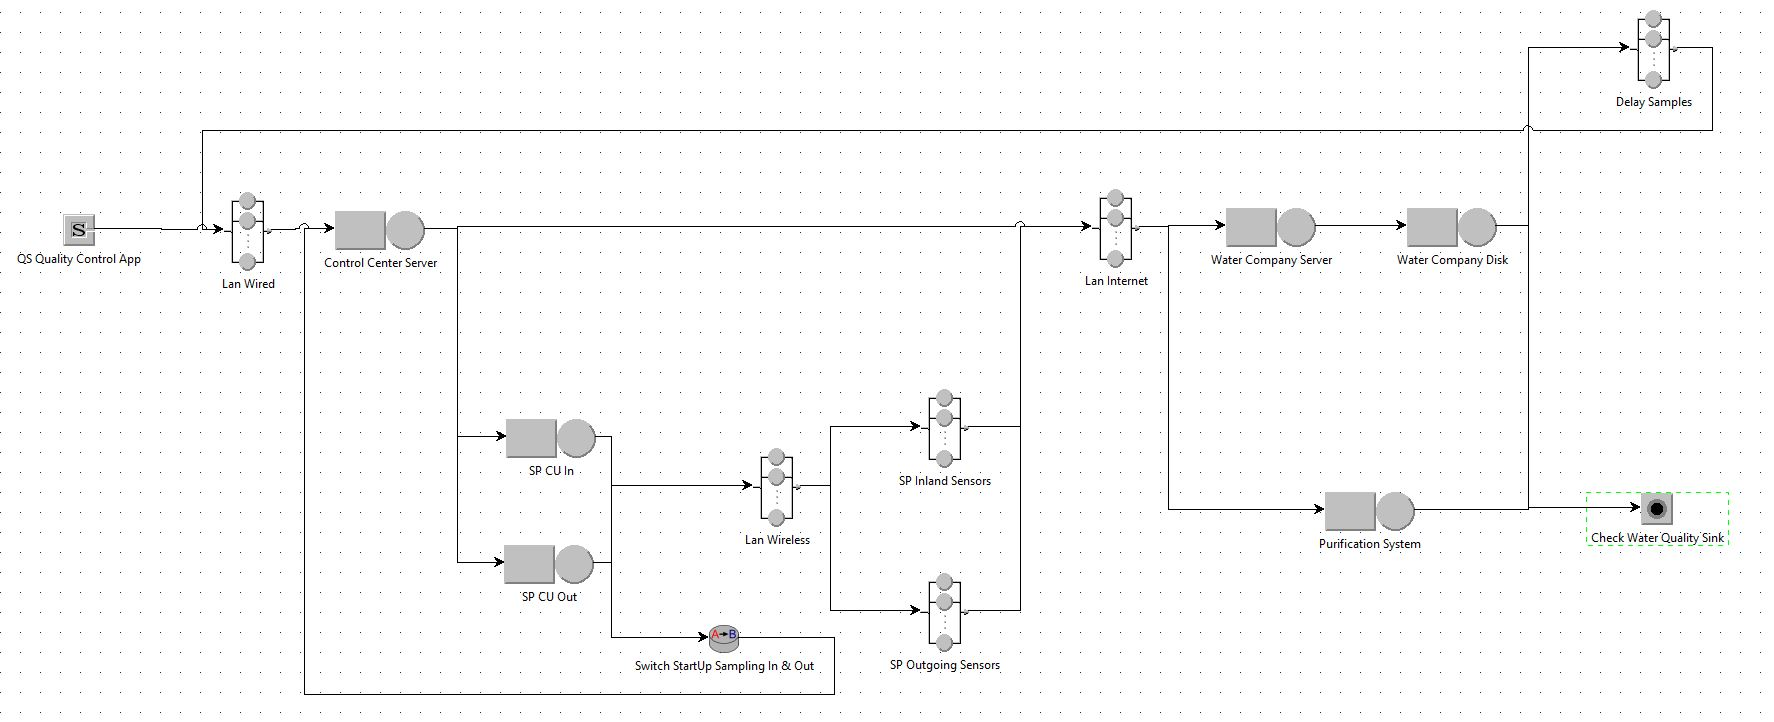
\includegraphics[width=\textwidth]				{QueuingNetworkFinal.jpg}}
\end{center}
\bigskip
\captionof{figure}{Final Queueing Network}
\chapter{\textbf{Parameterization}}

In order to have a mapping beetwen the consumption of our Physical Resources and Virtual Resources we identified a Overhead Matrix:

\begin{center}
\makebox[\textwidth]{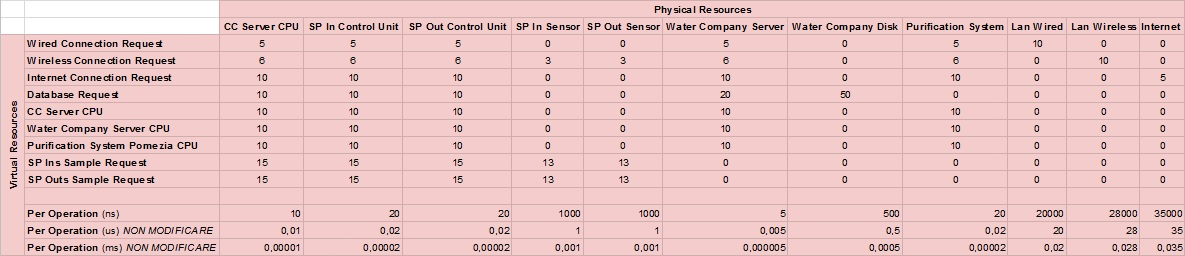
\includegraphics[width=\textwidth]
{1-OverheadMatrix.jpg}}
\end{center}
\captionof{figure}{Overhead Matrix}
\bigskip

In the last three rows of the table are specified the service time for Physical Resources to execute a basic operation.\\
The next step is obtain the whole consumption of our Virtual Resources for each Execution Graph considering the meaning of each individual block:

\begin{center}
\makebox[\textwidth]{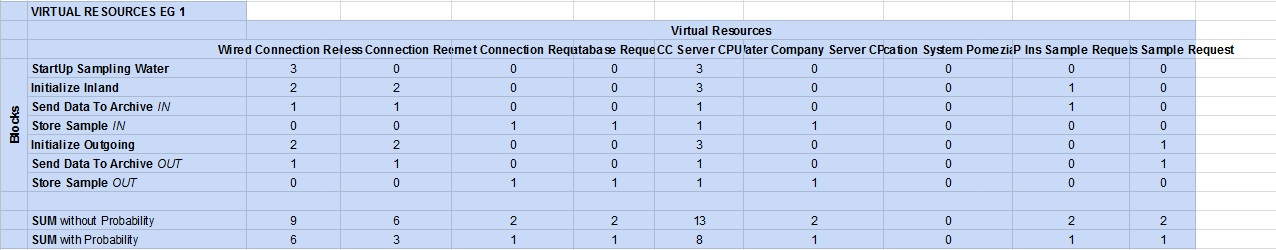
\includegraphics[width=\textwidth]
{2-VirtualResUsagebyeachNode.jpg}}
\end{center}
\captionof{figure}{Virtual Resource Usage By Each Block}


\begin{center}
\makebox[\textwidth]{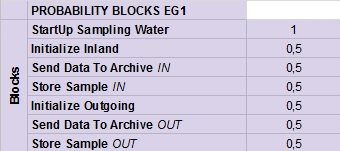
\includegraphics[width=7cm]
{3-Probeachnode.jpg}}
\end{center}
\captionof{figure}{Block Probability}
\bigskip

Considering this last table with the overhead matrix we obtain a matrix containing the consumption of the physical resources related to the considered Execution Graph. This method was applied for both execution graphs and then we reapplied it once we decided to split the jobs.

\begin{center}
\makebox[\textwidth]{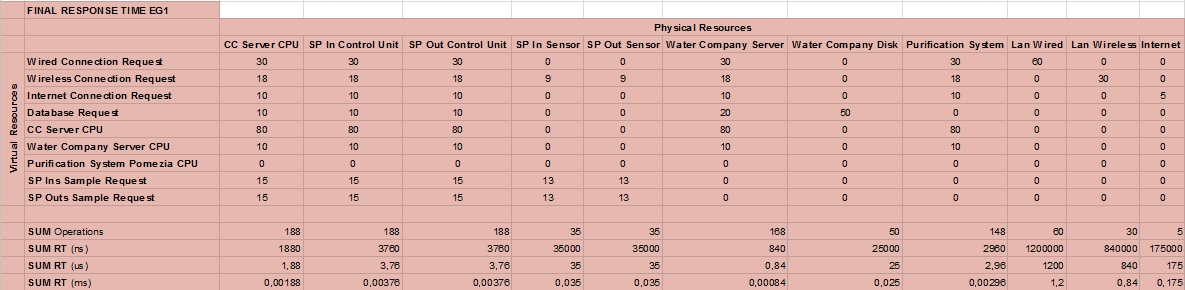
\includegraphics[width=\textwidth]
{4-FinalRes.jpg}}
\end{center}
\captionof{figure}{Final Resources Consumption}

Having introduced two differnt classes of jobs, for the same reasons expressed in the chapter 8, wh have also to re-evaluate the service demand of the new classes of jobs. 
For more details we refer to the attached excel files.

Related file is JMT\ Project/Parametrization.xlsx
\chapter{\textbf{Queueing Network Solving And BottleNeckAnaliysis}}

Once parameterized the Queueing Network, the data was inserted into Java Modelling Tool (JMT). It was decided to carry out a simulation with a number of SeaweedPickingInland/Outgiung equal to one thousand for each.\\
Various output Indices were analyzed in first analysis.
Performance Indices:
\begin{itemize}
\item Utilization:
	\begin{itemize}
		\item Control Center Server;
		\item SeaweedPicking Control Unit;
		\item Water Company Server;
		\item Purification System;
		\item Water Company Disk.
	\end{itemize}
\item Response Time:
	\begin{itemize}
		\item Control Center Server;
		\item SeaweedPicking Control Unit;
		\item Water Company Server;
		\item Purification System;
		\item Water Company Disk.
	\end{itemize}
\item Response Time Sink (Check Water Quality);
\item Throughput for Sink (Check Water Quality).
\end{itemize}

It resulted that the simulation was successful for all performance
indices. Then we choose to run multiple simulations with increasing
number of sensors to understand how the system scales and how it
respond to the increasing of inputs. For this purpose we have done a What-If simulation composed of one hundred sub-simulation and it has come out that the Utilization performance of the Control Center Server, Water Company Disk gets worse when the fourteen thousand sensors are reached.\\
Other proof of this is the analysis of the Response Time.

\section{Refactoring}

For the refactoring phase we wanted to consider the case in which we want to increase the number of Seaweed Picking to twenty thousand units. in this case, as we saw in the previous analysis, we have a bottleneck linked to the Control Center Server and to the Water Company Disk.

\begin{itemize}
	\item Software Solution;
	\item Hardware Solution.
\end{itemize}

We have chosen a hybrid solution because we have halved the service time for each class of jobs for the Water Company Disk and for the Control Center Server, and decided to have two separate Water Company Disks one for the Sample Inland and one for the Sample Outgoing that translates into a modification of the architecture.\\
In addition, by resolving the new model we noticed an unexpected increase in the use of SCPU and for this reason we have slightly reduced the service time of this node.
\chapter{\textbf{AEmilia Model}}

The model implemented by us in Aemilia is modeled in a phase prior to refactoring.

\section{Work Planning}

The workflow was:
\begin{itemize}
\item Study of theoretical concepts of Aemilia;
\item Drafting of Flow Graph;
\item Drafting of State Diagram;
\item Implementation of the Model;
\item Test and Analysis of results.
\end{itemize}

\section{Aemilia Flow Graph}

A Flow Graph represents the topology of an architecture described in AEmilia. It is convenient to start with the flow graph representation of the architectural type and then to specify the behavior of each node.  

\begin{center}
  \makebox[\textwidth]{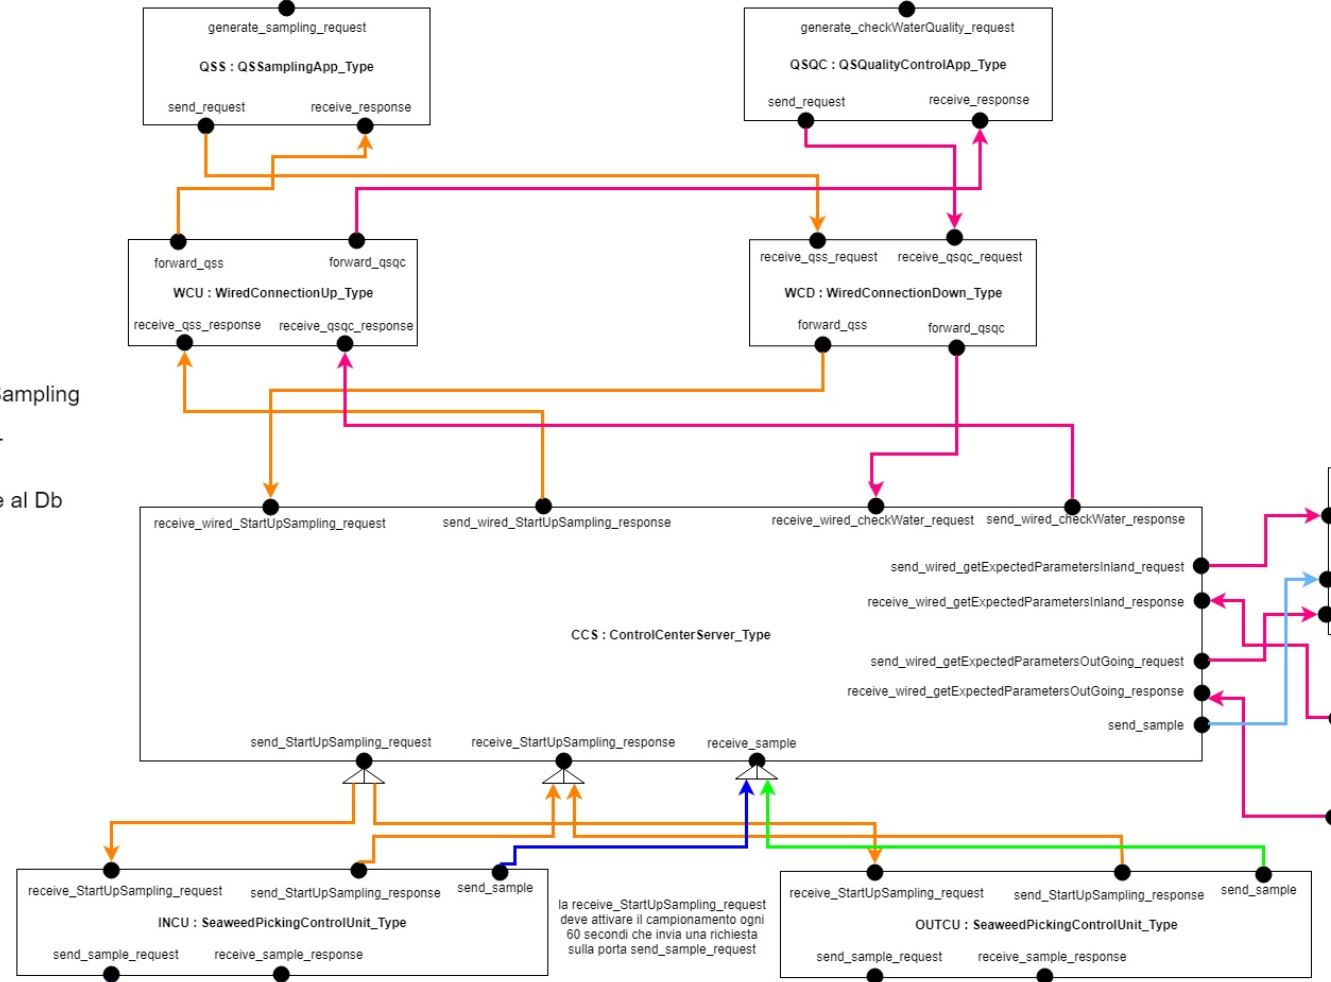
\includegraphics[width=\textwidth]{schermata1.JPG}}
\end{center}
\bigskip
\captionof{figure}{Flow Graph Extract}

\section{Aemilia State Diagram}

In describing the behavior, we created our Diagrams for each Node of the Flow Graph.

\begin{minipage}{0.3\textwidth}
\bigskip
  \makebox[\textwidth]{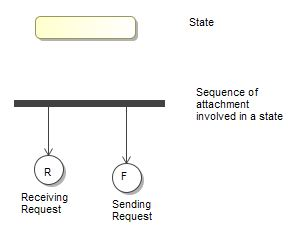
\includegraphics[width= 8cm]				{Legenda.JPG}}
\captionof{figure}{Legenda}
\end{minipage}
\hfill
\begin{minipage}{0.4\textwidth}\raggedleft
We have a block representing the state, a fork under which there is a
sequence of attachments involved within the same state, two circumferences representing these attachments
\end{minipage}
\bigskip

Below you can see an extract of it:

\begin{center}
  \makebox[\textwidth]{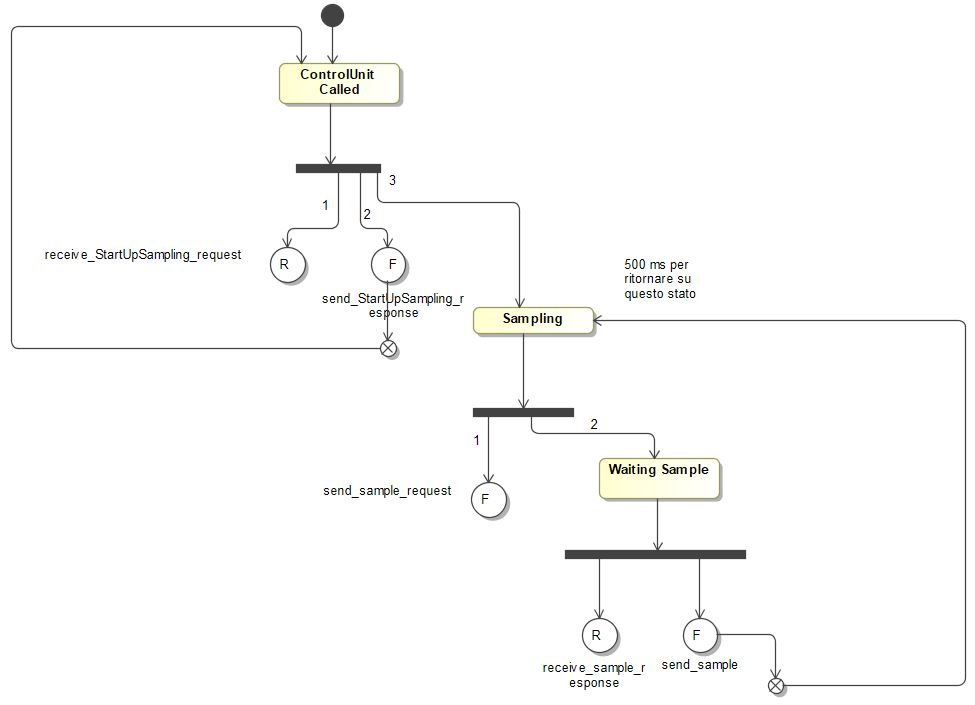
\includegraphics[width=\textwidth]				{stateDiagram.JPG}}
\end{center}
\bigskip
\captionof{figure}{State Diagram Extract}
\bigskip

In this image we see the behavior of the component "SeaweedPicking Control Unit." 


\section{Implementation Of The Model}

\subsection{Two Towers's Performance Evaluator limits}

To simulate the presence of 1000 sensors in and out we came across a variety of problems that forced us to vary the model and its implementation. The initial idea was to have in the Flow Graph 1000 instances of the Architecture Element Type "Sensor Type" incoming and outgoing, but in the next phase of the perfect evaluator Two Towers notified us that the size of the Markov Chain was too large.\\
Subsequently to overcome this limitation we thought to have a single sensor in input and output whose Delay Rate was increased by a factor open to the number of sensors in input and output that we wanted to have previously.\\
We made this choice because we thought that having only one sensor whose short wait was the closest possible to have a number of distinct sensors with a greater wait so as to stress the system in equal way.\\
Another problem encountered was that of stressing the system with the presence, as in jmt, of a population of 1000 jobs of the type of StartUp Sampling Water Inland and Outgoing. In fact, we initially tried to generate exactly 1000 StartUp messages with a buffer, but the Perfomance Evaluator in Two Towers never seemed to arrive at a solution in an acceptable time.\\
At this point we adopted the choice of having a single activation of the two StartUps aware of the fact that it was not the best choice as far from the real scenario, but compared to the simulation performed in jmt, we knew that the workload on the system of these it was not excessively large\\

\subsection{Implementation Code}

Once the behavior of the various nodes, the architecture has been written following the syntax of Aemilia. Below, we will be proposed snippets, coming from previous pictures. 

\lstset {language = C}
\bigskip
\begin{lstlisting}
ELEM_TYPE SeaweedPickingControlUnit_Type(const rate SPCU_send_StartUpSampling_response_rate, const rate SPCU_send_sample_request_rate, 
	const rate SPCU_send_sample_rate, const rate SPCU_delay_rate, const integer sensors_num)

BEHAVIOR

	ControlUnitCalled(void;void) = 
		<receive_StartUpSampling_request, _> . <send_StartUpSampling_response, exp(SPCU_send_StartUpSampling_response_rate)> . Sampling();

	Sampling(void;void) = 
		<send_sample_request, exp(SPCU_send_sample_request_rate)> . WaitingSample();

	WaitingSample(void;void) = 
		<receive_sample_response, _> . <send_sample, exp(SPCU_send_sample_rate)> . Delay();

	Delay(void;void) =
		<delay, exp(SPCU_delay_rate * sensors_num)> . Sampling()


INPUT_INTERACTIONS

	UNI receive_StartUpSampling_request;
		receive_sample_response

OUTPUT_INTERACTIONS 

	UNI send_StartUpSampling_response;
		send_sample;
		send_sample_request
\end{lstlisting}

\section{Test And Analysis Of Results}

After building the model, it was written a file describing the
performance measures to be analyzed. 

\lstset {language = C}
\bigskip
\begin{lstlisting}
MEASURE SeaweedPickingINControlUnitUtilization IS
	ENABLED(INCU.send_StartUpSampling_response) -> TRANS_REWARD(1)
	ENABLED(INCU.send_sample) -> TRANS_REWARD(1)
	ENABLED(INCU.send_sample_request) -> TRANS_REWARD(1);
\end{lstlisting}

After simulating the Model the results are this:

\lstset {language = C}
\bigskip
\begin{lstlisting}
- Value of measure "ControlCenterServerUtilization":
	0.003647

- Value of measure "WaterCompanyServerUtilization":
	0.00271904

- Value of measure "WaterCompanyDiskUtilization":
	0.00225506

- Value of measure "SeaweedPickingINControlUnitUtilization":
	0.0017911

- Value of measure "SeaweedPickingOUTControlUnitUtilization":
	0.0017911

- Value of measure "PurificationSystemServerUtilization":
	0.000463978
\end{lstlisting}

%%Controllare e modificare frase nel caso
As can be seen from the results the values obtaines from the Aemilia simulation are close to those of JMT  exept for the Water Company Disk and the non functional requirements specified at the beginning are all respected.\\

\subsection{Bottelneck Test}

In a second phase we increased the number of sensors by the same number for which we had the bottoleneck on the Water Company Disk on jmt but from the results of the simulation with Aemilia we did not have a worse use of the aforementioned node significantly so as to highlight the presence of a Bottleneck.\\
For this reason we tried to increase the number of sensors in a significant way but from the results of the simulation we noticed that the utilization of the system did not increase beyond a certain threshold and for this we assumed the presence of an asymptote.

\subsection{Another Modeling Attempt}


Not satisfied with the results of the previous simulations we have made a further model not starting from the deployment and the sequence diagram but from the queueing network. We know that this choice is wrong because we treat two different models but we wanted a comparison with the simulations performed on jmt.\\
In the image below you can see the new Flow Graph:

\begin{center}
	\makebox[\textwidth]{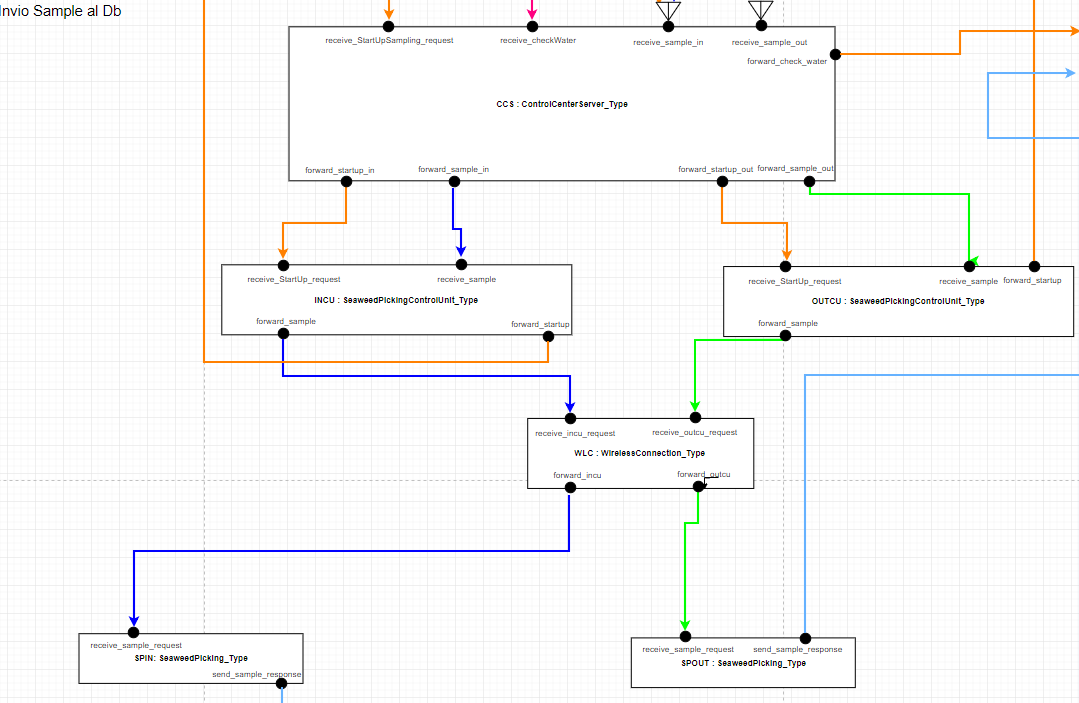
\includegraphics[width=\textwidth]	{Aemiliacomejmt.PNG}}
\end{center}
\bigskip
\captionof{figure}{Flow Graph Extract}
\bigskip

But also in this case the simulation results both with 1000 inland and outgoing sensors and for the number of sensors for which the bottleneck should be presented on the Water Company Disk are not comparable to those of jmt.\\

\begin{lstlisting}
%%%%%%%%%%%%%%%%%%%%%%%%%%%%%%%%%%%%%%%%%%%%%
%	1000 in & 1000 out						%
%%%%%%%%%%%%%%%%%%%%%%%%%%%%%%%%%%%%%%%%%%%%%

Stationary value of the performance measures for wcs:

- Value of measure "ControlCenterServerUtilization":
0.0197883

- Value of measure "WaterCompanyDiskUtilization":
0.0340923

%%%%%%%%%%%%%%%%%%%%%%%%%%%%%%%%%%%%%%%%%%%%%
%	4000 in & 4000 out						%
%%%%%%%%%%%%%%%%%%%%%%%%%%%%%%%%%%%%%%%%%%%%%

Stationary value of the performance measures for wcs:

- Value of measure "ControlCenterServerUtilization":
0.0207671

- Value of measure "WaterCompanyDiskUtilization":
0.0351357
\end{lstlisting}


Against this we came to the conclusion that the subsystem we considered was not comparable between jmt and Aemilia.
\chapter{\textbf{Our Conclusion}}

With this second homework we have been able to fully understand the importance of the analysis and validation of UML models on the basis of functional requisites using methods and tools such as queueing Network and Descrption Language For Performance Analsiys like Aemilia.
So we leave this experience with an enriched baggage that we hope will be useful for us in a future working environment

\end{document}
